\documentclass[10pt]{article} % For LaTeX2e
\usepackage{nips14submit_e,times}
\usepackage[letterpaper, margin = 1in]{geometry}
\usepackage{hyperref}
\usepackage{url}
\usepackage{graphicx}
\usepackage{float}
\usepackage{amsmath, amssymb}
\usepackage{array}


\title{Eyes Around The World - Learning to Alert and Cluster Live Webcams}


\newcommand{\fix}{\marginpar{FIX}}
\newcommand{\new}{\marginpar{NEW}}


\begin{document}
\maketitle

%\begin{abstract}
%Fill in abstract if there is space.
%\end{abstract}

\section{Introduction}
There are a large number of public live webcams that are accessible over the internet. A variety of content and objects from various places all around the world are being recorded by these webcams in real-time, but it is not feasible for a single person to browse through all of the webcams to search for content that is of interest. Our project aims to use Machine Learning algorithms to cluster and identify webcams of interest out of a large pool of webcams. This has relevance to security, surveillance and exploration applications where there is a need to filter through a large number of video streams to detect objects of interest. 

The input to our system is a stream of images from multiple webcams. For each webcam image, we use a Gaussian mixture model to model the background image, use to background model to extract foreground objects from the webcam image, and use a convolutional neural network to classify the detected objects. The output of our system is a display list of the top 5 webcams as ranked by the scoring algorithm for the webcams, which can be changed depending on the user input query. We also use K-means clustering to explore the different categories of webcams that exist in our dataset. 

\section{Related Work}
Several groups have previously looked at exploring and characterizing the network of webcams around the world. A previous effort was made to discover and characterize the locations and categories of webcams \cite{webcamnetwork} based on their geo-IP addresses and links from existing GIS databases. Our current work extends this effort to try to characterize webcams where there does not exist clean metadata and descriptions of the webcams. There has also been work in the area of image fusion \cite{billioneyes} of webcam images with data from Google StreetView and Google Earth images to provide additional context to existing images from a webcam. This was more aimed towards providing improved location-based services for mobile applications, whereas our work focuses on alerting webcams solely based off their data streams. 

The closest and most relevant previous work that has been conducted is real-time abnormality detection from multiple webcams \cite{huntingnessie}, where a nearest-neighbor model is used to create a image abnormality classifier based on simple image features. The distance/similarity metric used for nearest-neighbors clustering is based on outliers relative to a sample of past webcam images from varying time intervals, and is primarily based on image quadrants in a picture. Our work extends this by showing that it is possible to use object tracking methods by working on a pixel level instead of a quadrant level to detect objects, and our work differs in that our interest metric is primarily tied to the activity of a scene instead of abnormality relative to past images. 

Other related work is person identification from webcam images via semi-supervised learning \cite{personidentification}, where facial features are extracted from webcam images to locate track the position of people in those images. Our approach differs from this aspect in that we aim to track multiple kinds of objects instead. Work has also been done in using webcams to detect and monitor birds in the wild \cite{birddetection} using a median filter by defining the background as the median of the previous N frames. Our work uses a different method (model background as Gaussian mixture model) for object detection instead. 

\section{Dataset and Features}
Our data set consists of images logged from approximately 2000 publicly accessible, non-password-protected webcams, where query urls were scraped from the website opentopia.com \cite{opentopia}. Although we would ideally run our algorithms directly on live webcam streams, the bandwidth required to simultaneously process a meaningful number of webcams was prohibitively high. As a result, we logged images from those 2000 webcams every 5 minutes over a period of 1 week, and ran our algorithms on that dataset. 

The raw webcam images vary greatly in resolution - From as low to 240 x 180 to as high as 2048 x 1536. We log the webcam images in their native resolution for processing flexibility later on, and resize them to smaller resolutions (typically 300 x 300) as input into our system. Sample images from some webcams are shown below:

The features varied for our initial attempts at clustering and in our main
effort of classification. For clustering, we used a Bag-of-Features model (akin
to the Bag-of-Words model which is common in language). The seed of these
features are SIFT descriptors. We will go more in depth about how we generated
these features in the Methods section. For classification, we used the patches
of images containing moving objects found through background subtraction as our
features. These patches were rescaled to 224 x 224 before being passed to the
network.

\begin{figure}[h]
\caption{Sample webcam images}
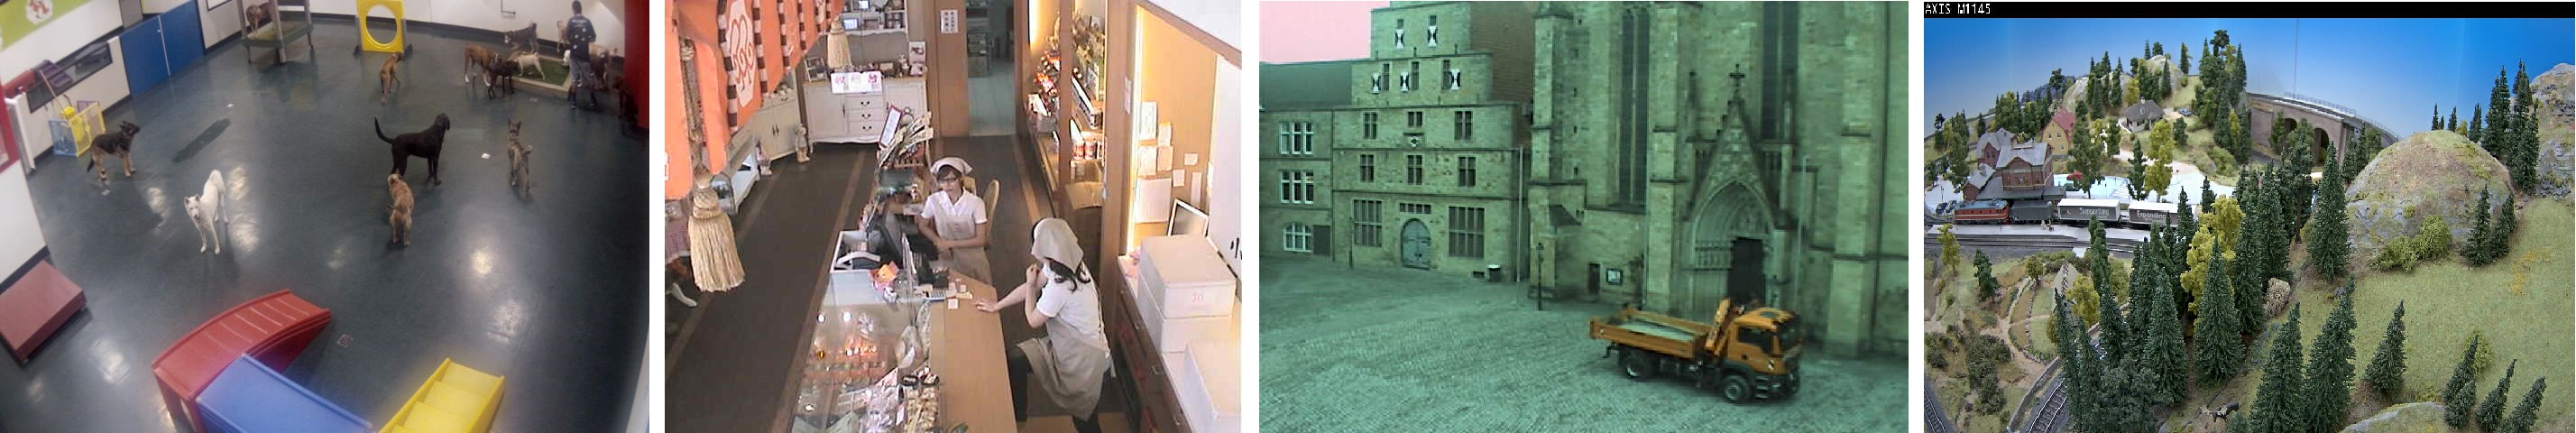
\includegraphics[scale = 0.25]{samples}
\end{figure}

\section{Methods}
\subsection{Webcam ranking}
In order to rank webcams based on the activity of the objects recorded, it is necessary to separate foreground objects from the image background. To do this, we use OpenCV's BackgroundSubtractorMOG2() method to construct a background model for each pixel, and use it to classify pixels as foreground or background. The method implements the algorithm described in a paper by Zivkovic \cite{zivkovic} for background subtraction. The model is a generative model that uses a Gaussian mixture model (GMM) to model the background color distribution for each pixel. 

Let $\vec{x}^{(t)}$ be the value of a pixel at time $t$, and let $T$ be a time period over which samples are recorded. Define the training data set $\chi_T = \{\vec{x}^{(t)}, ... ,\vec{x}^{(t-T)}\} $. $\chi_T$ is updated with each new sample. An estimate of the background (BG) and foreground (FG) distribution can be modeled by a GMM with $M$ components :
\begin{equation}
\hat{p}(\vec{x}^{(t)} | \chi_T , BG+FG) = \sum_{m=1}^M \hat{\pi}_m \mathcal{N}(\vec{x} ; \hat{\vec{\mu}}_m ,  \hat{\sigma}_m^2 I)
\end{equation}
where $\hat{\vec{\mu}}_1 , .. , \hat{\vec{\mu}}_m$ are mean estimates and $\hat{\sigma}_1 , ... , \hat{\sigma}_m$ are variance estimates. $\hat{\pi}_m$ are the mixing weights that are non-negative and sum to 1. Given a new data sample $\vec{x}^{(t)}$, the parameters of the model can be updated recursively as \cite{zivkovic2}:
\begin{equation}
\hat{\pi}_m \leftarrow \hat{\pi}_m + \alpha ( o_m^{(t)} - \hat{\pi}_m) \\
\end{equation}
\begin{equation}
\hat{\vec{\mu}}_m \leftarrow \hat{\vec{\mu}}_m + o_m^{(t)} (\alpha / \hat{\pi}_m) \vec{\delta}_m \\
\end{equation}
\begin{equation}
\hat{\sigma}_m^2 \leftarrow + o_m^{(t)} (\alpha / \hat{\pi}_m)(  \vec{\delta}_m^T  \vec{\delta} - \hat{\sigma}_m^2)
\end{equation}
where $\vec{\delta} = \vec{x}^{(t)} - \hat{\vec{\mu}}_m$,  $\alpha$ is a exponential decay factor such that $\alpha \approx 1/T$ to limit influence of old data, and $o_m^{(t)}$ is defined as the "ownership". For a new sample, $o_m^{(t)}$ is set to 1 for the 'closest' component with largest $\hat{\pi}_m$ and others are set to zero, where 'closest' is based on the mahalanobis distance metric. The squared distance from the $m$-th component is calculated as $D_m^2 ( \vec{x}^{(t)}) = \vec{\delta}_m^T  \vec{\delta} / \hat{\sigma}_m^2$. 

Foreground objects usually correspond to some additional clusters with small weights $\hat{\pi}_m$. Thus, the background model can be approximated by the first $B$ largest clusters
\begin{equation}
p(\vec{x} | \chi_ , BG) \sim \sum_{m=1}^B \hat{\pi}_m \mathcal{N}(\vec{x} ; \hat{\vec{\mu}}_m ,  \hat{\sigma}_m^2 I)
\end{equation}

We use the background model to classify each pixel in the image as either being part of the foreground or background to obtain a foreground mask. We then fit contours around the sections of foreground object pixels using OpenCV's findContours() method. The contours are filtered based on size - Contours that are too small ($<$ 1\% of picture area) are attributed to noise, contours that are too large ($>$20\% of picture area) are attributed to pixel changes due illumination or webcam position, which are not of interest. \textcolor{red}{Example pics?}

A webcam's score is then calculated as the sum of contour areas as a percentage of the image size divided by the sum of contour arc lengths, Score = total contour area % / total contour length. We maximize for contour area to be able to show the largest / most number of objects after filtering. We minimize for contour length to reward convexity, as we found that large noisy artifacts in the webcam images tended to be highly non-convex in shape. \textcolor{red}{Example pics?}

\subsection{Clustering}
The most involved operation in clustering our webcams was extracting the
features. We wanted to capture semantic information about the webcams, and
therefore needed features which captured semantic information from frames. We
decided to base our features off of SIFT descriptors \cite{lowe}. These
descriptors are scale, translation, and rotation invariant. Furthermore, they
are robust to lighting changes or slight deformation. These properties are
desirable for our application, as objects will appear under different
conditions in our webcams. Given an image, one can extract multiple SIFT
descriptors, each of which corresponds to some local feature of the image. Each
descriptor is a vector in $\mathbb{R}^{128}$.

With this machinery, we will illustrate a method for extracting features from
each webcam. First, we generate the \textit{visual vocabulary} by first
sampling random frames from every webcam and extracting SIFT descriptors, and
then clustering the descriptors using k-means. The resulting cluster centroids
are the words in our vocabulary. Then, we compute the feature vectors for each
webcam by extracting SIFT descriptors fram a random subset of frames from each
webcam and computing a histogram of the closest vectors in the vocabulary to
the descriptors we extracted. The resulting histogram is the feature we use to
represent the webcam.

Finally, we cluster the webcams' corresponding features using k-means using
initial clusterings chosen by k-means++. In k-means++, each initial cluster
center is chosen from a weighted distribution over the dataset, where the
weight corresponding to a certain point is the squared distance between that
point and the closest initial centroid we have chosen so far. The first initial
centroid is chosen uniformly at random from all of the points. The resulting
clusters are the different unlabeled categories for our webcams.

\subsection{Convolutional Neural Network}
\subsubsection{Network}
We used modified version of the BLVC Reference CaffeNet, which is a slightly
modified version of AlexNet \cite{krizhevsky}. This network features around 60
million parameters and 500,000 neurons. There are five convolutional layers,
some of which are followed by max-pooling layers, then two fully connected
layers, and finally a 3-way softmax.  The only difference between our network
and the BLVC Reference CaffeNet is that our softmax layer produces 3 outputs,
whereas theres produces 1000.
\subsubsection{Dataset}
Our dataset consists of hand-labeled patches from a random subset found using
our previously described moving object detector. This dataset consists of 9776
examples total, 142 (1.453\%) of which are humans, 249 (2.547\%) of which are
vehicles, and 9385 (96.000\%) of which are noise. We separated this into a
training set and a testing set. The training set consists of 90\% examples
randomly sampled from each class, and the test set consists the remaining
examples.
\subsubsection{Training}
We fine-tuned the pretrained BLVC Reference CaffeNet on our dataset. The model
was pretrained on the ILSVRC 2012 dataset by Jeff Donahue. We then fine-tuned
the model on our dataset, using a base learning rate of 0.001 for the original
layers and a learning rate of 0.02 for the final softmax layer. We
trained the network for a few hours using a single 980 TI.



\textcolor{red}{[SEAN: Add mathematical formulations for clustering and CNN if room]}

\section{Results / Discussion}
\subsection{Webcam ranking}
We present 2 sample snapshot results of the top 4/1000 webcams as ranked by our scoring algorithm. The webcam images with detected objects is shown on the top row, and the corresponding background image is shown in the bottom row. 
\begin{figure}[H]
\centering
\caption{Snapshot of top 4/1000 webcams from run 1 (left) and run 2 (right)}
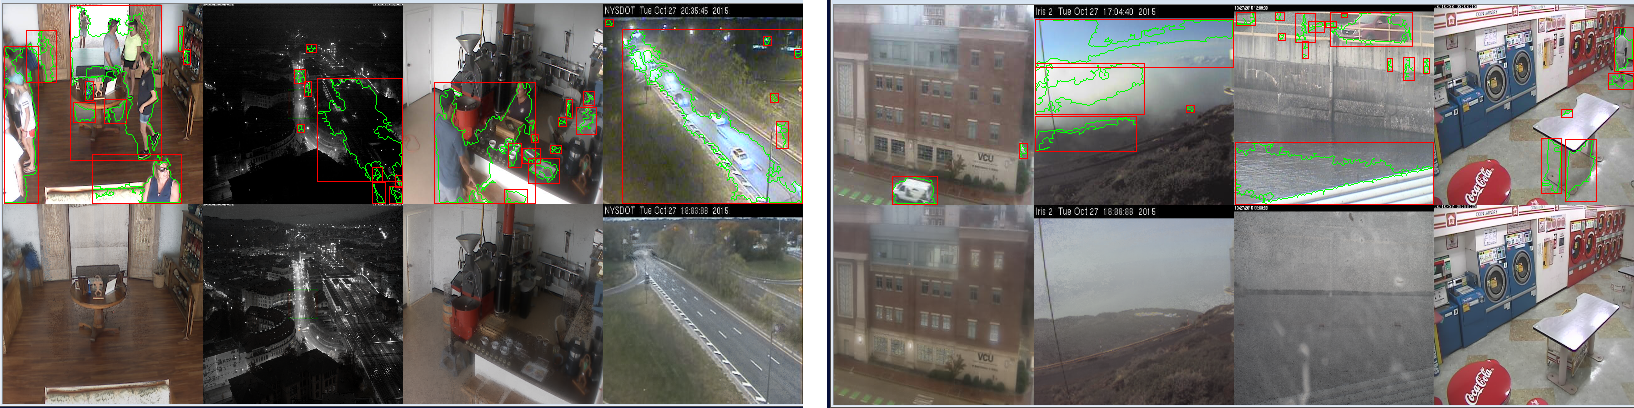
\includegraphics[scale = 0.5]{wc}
\end{figure}
We see that the algorithm returns qualitatively acceptable results - It is able to highlight clear changes and rise in activity of webcams, such as people filling into a room or traffic conditions changing. 

Even though we perform filtering on contours and on the scoring function to try to eliminate noise, there are still occurrences where our algorithm is influenced by image, lighting or webcam noise and ranks certain webcam images highly when there actually isn't any noticeable activity or changes. Several examples of webcam images that were ranked in the top 5/1000 are shown below :
\begin{figure}[H]
\centering
\caption{Examples of erroneously highly-ranked webcam images}
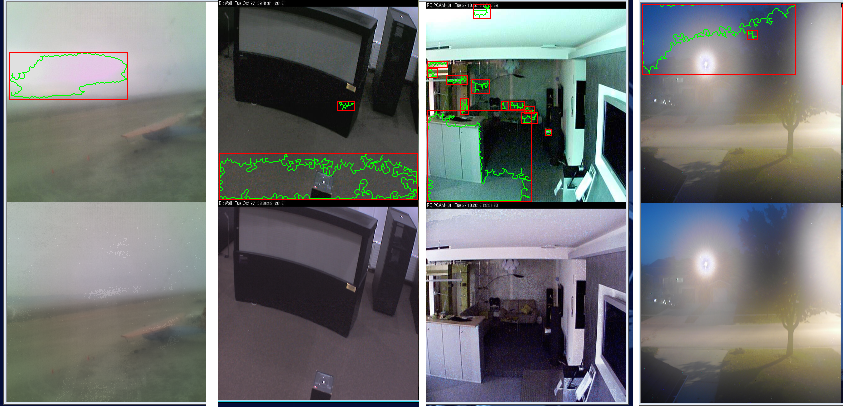
\includegraphics[scale = 0.5]{fails}
\end{figure}

\section{Clustering}
The results of clustering were lackluster. We found that the number of clusters
played a large role in the expressiveness of the clusters. Too many clusters
produced overly noisy clusters. Too few clusters produced overly broad
clusters. With a moderate number of clusters, we did see some meaningful
categories. For instance, we produced an animal cluster, which contained images
of cats and dogs. However, this category was not exclusive. While it contained
a disproportionately large number of webcams featuring webcams, it also
contained unrelated webcams. While the clustering did produce some clear
results, we deemed them to be too noisy for useful categorization.

\section{CNN Filtering}
Our filtering results were promising. We have three primary interests. First,
we want to filter out as many noisy detections as possible.  Secondly, since
there are proportionally few examples of vehicles and humans, a high recall
percentage was desirable. Third, we wanted to use the convnet for search and
clustering, so precision was also important. Our CNN produced the following
results on the held-out test set:
\begin{center}
  \begin{tabular}{ | m{5em} | m{5em}| m{5em} | m{9em} | m{13em} | } 
    \hline
    Class & Precision & Recall & Percentage of Dataset & Percentage of Filtered Dataset  \\ 
    \hline
    Human & 69.2\% & 64.3\% & 1.453\% & 28.7\%  \\ 
    \hline
    Vehicle & 73.9\%  & 68.0\% & 2.547\% & 48.6\% \\ 
    \hline
    Noise & 97.8\%  &99.1\% & 96.000\% & 22.9\%  \\ 
    \hline
  \end{tabular}
\end{center}

For our applications, these results are extremely useful. High precision and
recall for objects of interest mean that searching and clustering are possible.
Although an even higher precision is desirable, our current numbers are still
high considering the dataset makeup. Furthermore, the filtered dataset only
contains 22.9\% noise, which is much lower than the original dataset which was
comprised of 96\% noise. Thus, the top-5 most interesting webcams are
significantly more likely to contain objects of interest when filtered.

Our network produced the following confusion matrix:
\begin{center}
  \begin{tabular}{ | m{8em} | m{5em}| m{5em} | m{5em} | }
    \hline
    & \multicolumn{3}{c|}{\textbf{Correct Label}} \\ 
    \hline
    \textbf{Predicted Label} & Human & Vehicle & Noise \\
    \hline
    Human & 0.692 & 0.0 & 0.308 \\
    \hline
    Vehicle & 0.043 & 0.739 & 0.217 \\
    \hline
    Noise & 0.004 & 0.008 & 0.987 \\
    \hline
  \end{tabular}
\end{center}
The confusion matrix tells us that incorrect predictions on humans and vehicles
are generally not helpful. That is, incorrect predictions usually lead to
inclusion of noise rather than an object of interest of another class.


\section{Conclusions / Future Work}
We have demonstrated a system to rank a large number of webcams using an interest metric that is based on the amount of activity that is currently recorded by a webcam. Webcam activity was quantified by the area of contours fit to foreground pixels classified by a Gaussian Mixture Model for the background model, and the interest metric was designed to reward the number, size and convexity of detected objects. 

One of the main bottlenecks to this project was the amount of GPU memory available to store webcam images. In order to be able to detect objects reliably, it is necessary to have the resolution of the images be above a certain size. However, the GPU memory required to process each image increases as the image resolution increases. At an image resolution of 300 x 300, we were able to simultaneously process a maximum of 1000 images at a time. Given extra computational resources, we would apply our system to the all 2000 webcams in the dataset.

There are a few avenues we can take in the future in regards to the CNN. First,
we could tweak the criteria for selecting which label to predict based on the
probabilities output by the network. Doing so could lead to better precision
and recall, or a better tradeoff between the two. If we were to go down this
route, I would propose that we shard our dataset so that we could dynamically
choose training, testing, and validation sets. Doing so would allow us to
validate the choices of the different hyperparameters. Furthermore, we could
collect more data as there are relatively few positive examples for both of our
objects of interest. This would give us better estimates of our metrics as well
as better generalization. Furthermore, we could support better clustering as
well as search by using the data filtered and labeled by the convnet.



\begin{thebibliography}{10}
\bibitem{webcamnetwork}
Jacobs, Nathan, et al. "The global network of outdoor webcams: properties and applications." Proceedings of the 17th ACM SIGSPATIAL International Conference on Advances in Geographic Information Systems. ACM, 2009.

\bibitem{billioneyes}
Luo, Jiebo. "Vision with a billion eyes." Proceedings of the 2nd ACM international workshop on Geotagging and its applications in multimedia. ACM, 2013.

\bibitem{personidentification}
Balcan, Maria-Florina, et al. "Person identification in webcam images: An application of semi-supervised learning." (2005).

\bibitem{huntingnessie}
Breitenstein, Michael D., Helmut Grabner, and Luc Van Gool. "Hunting nessie-real-time abnormality detection from webcams." Computer Vision Workshops (ICCV Workshops), 2009 IEEE 12th International Conference on. IEEE, 2009.

\bibitem{birddetection}
Verstraeten, Willem W., et al. "Webcams for bird detection and monitoring: A demonstration study." Sensors 10.4 (2010): 3480-3503.

\bibitem{opentopia}
"Opentopia." Opentopia. Web. 10 Dec. 2015.

\bibitem{zivkovic}
Zivkovic, Zoran. "Improved adaptive Gaussian mixture model for background subtraction." Pattern Recognition, 2004. ICPR 2004. Proceedings of the 17th International Conference on. Vol. 2. IEEE, 2004.

\bibitem{zivkovic2}
Z.Zivkovic and F.van der Heijden, “Recursive Unsupervised Learning of Finite Mixture Models”, IEEE Trans. on PAMI, vol.26., no.5, 2004.

\bibitem{lowe}
Lowe, David. "Distinctive Image Features from Scale-Invariant Keypoints". (2004)

\bibitem{krizhevsky}
Krizhevsky, Alex. "ImageNet Classification with Deep Convolutional Neural Networks." Advances in Neural Information Processing Systems 25 1097-1105. NIPS, 2012.




\end{thebibliography}

\end{document}
